\chapter{Estimation Process}

\label{ch: Estim}

The parameter estimation problem can be interpreted as a optimization problem, where one must find the optimal values of parameters in order to reduce the error between real system and model. During the years, many methods were developed to address this problem, but two approaches have been largely employed to obtain its solution. 

The first approach applies metaheuristics to obtain a sufficiently good solution. These methods are used in a variety of cases, ranging from biological to engineering problems, due to the fact that they are not developed for a specific type of problem. Metaheuristics employ a stochastic search to encounter (near-)optimal solutions within a given region \cite{Blum2003}. Examples of metaheuristics are Ant Colony Optimization (ACO), Differential Evolution (DE), Particle Swarm Optimization (PSO) and Genetic Algorithm (GA). Applications of this approach in electrical power system cases can be found in \cite{•} and \cite{•}

\begin{figure}[h]
	\caption{Flowchart of estimation method}
	\begin{center}
		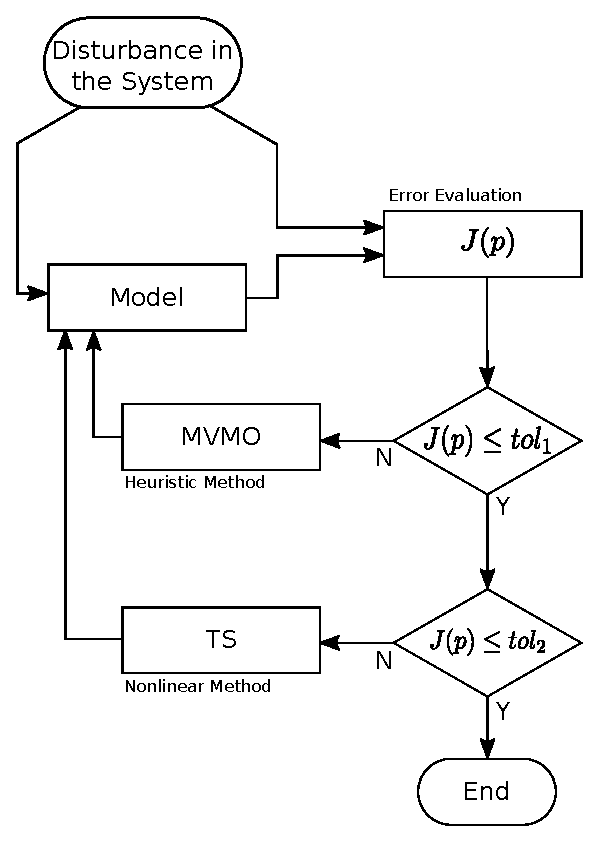
\includegraphics[scale=0.7]{Images/Flowchart.eps}
	\end{center}
	\label{fig: flowchart}
\end{figure}